\documentclass[12pt,letterpaper]{article}
\usepackage[utf8]{inputenc}
\usepackage[english]{babel}
\usepackage{listings}
\usepackage{xcolor}
\usepackage{graphicx}

%For syntax highlighting
\definecolor{codegreen}{rgb}{0,0.6,0}
\definecolor{codegray}{rgb}{0.5,0.5,0.5}
\definecolor{codepurple}{rgb}{0.58,0,0.82}
\definecolor{backcolour}{rgb}{1,1,1}

%%Sets different parameters
\lstdefinestyle{mystyle}{
	backgroundcolor=\color{backcolour},   
    commentstyle=\color{codegreen},
    keywordstyle=\color{magenta},
    numberstyle=\tiny\color{codegray},
    stringstyle=\color{codepurple},
    basicstyle=\ttfamily\footnotesize,
    breakatwhitespace=false,         
    breaklines=true,                 
    captionpos=b,                    
    keepspaces=true,                 
    numbers=left,                    
    numbersep=5pt,                  
    showspaces=false,                
    showstringspaces=false,
    showtabs=false,                  
    tabsize=4
}
\lstset{style=mystyle}

\title{\textbf{Department of Computer Science and Engineering}}
\author{\textbf{S.G.Shivanirudh , 185001146, Semester VI }}

\date{25 February 2021}

\begin{document}
\maketitle
\hrule
\section*{\center{UCS1611 - Internet Programming Lab}}
\hrule 
\bigskip\bigskip

%Assignment name
\section*{\center{\textbf{Ex 04: Java Servlets and MySQL}}}

%Objective
\subsection*{\flushleft{Objective:}}
\begin{flushleft}
    Write a servlet program whichreads all form details, finds the gross pay based on basic pay and designation. 
    The servlet returns all details (a-j, gross pay)in table format to the client.
\end{flushleft}

%Code
\subsection*{\flushleft{Code:}}
\subsubsection*{\flushleft{HTML:}}
\begin{flushleft}
\lstinputlisting[language = HTML]{employee/index.html}
\end{flushleft}

\subsubsection*{{\flushleft{Stylesheet:}}}
\begin{flushleft}
    \lstinputlisting[language = HTML]{employee/styles.css}
\end{flushleft}

\subsubsection*{{\flushleft{Script file:}}}
\begin{flushleft}
    \lstinputlisting[language = HTML]{employee/script.js}
\end{flushleft}

\subsubsection*{{\flushleft{Java file:}}}
\begin{flushleft}
    \lstinputlisting[language = Java]{employee/Servlet.java}
\end{flushleft}

\subsubsection*{{\flushleft{Java stylesheet:}}}
\begin{flushleft}
    \lstinputlisting[language = HTML]{employee/styles_servlet.css}
\end{flushleft}

\subsubsection*{{\flushleft{XML file:}}}
\begin{flushleft}
    \lstinputlisting[language = XML]{employee/WEB-INF/web.xml}
\end{flushleft}

\newpage
%Output
\subsection*{\flushleft{Output:}}
\begin{figure}[h]
    \centering
    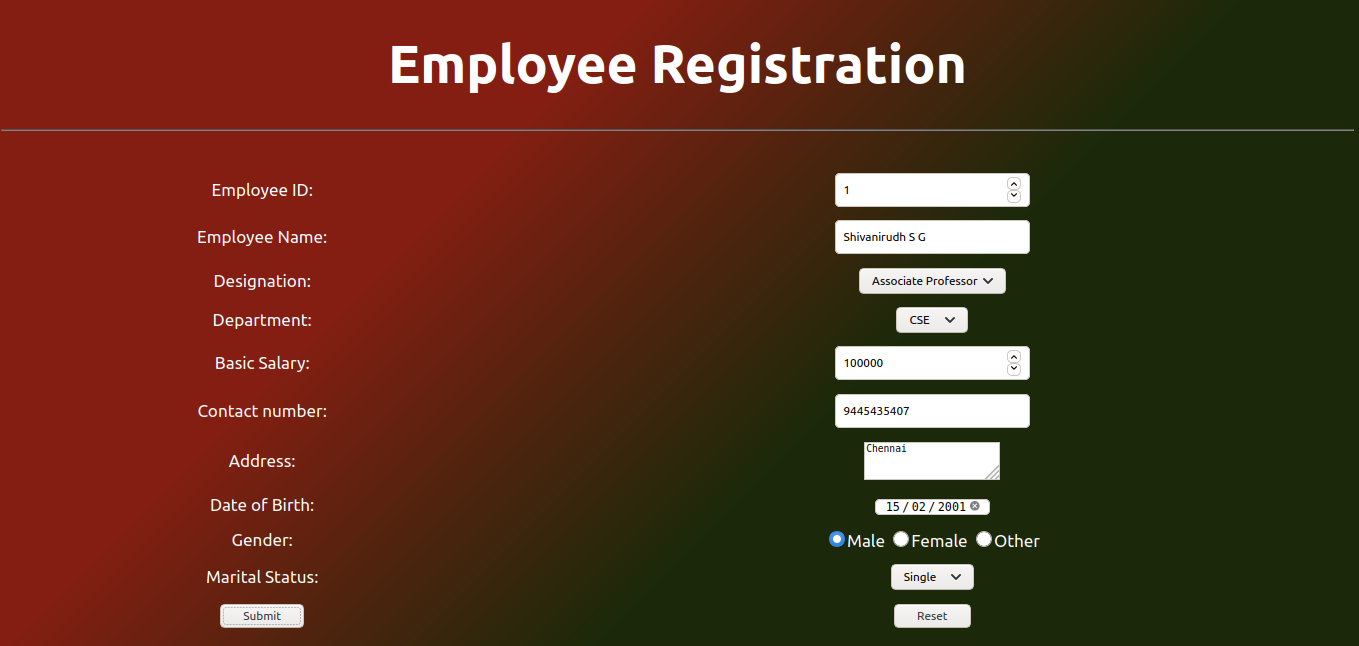
\includegraphics[width = \textwidth]{Pics/reg1.png}
\end{figure}
\begin{figure}[h!]
    \centering
    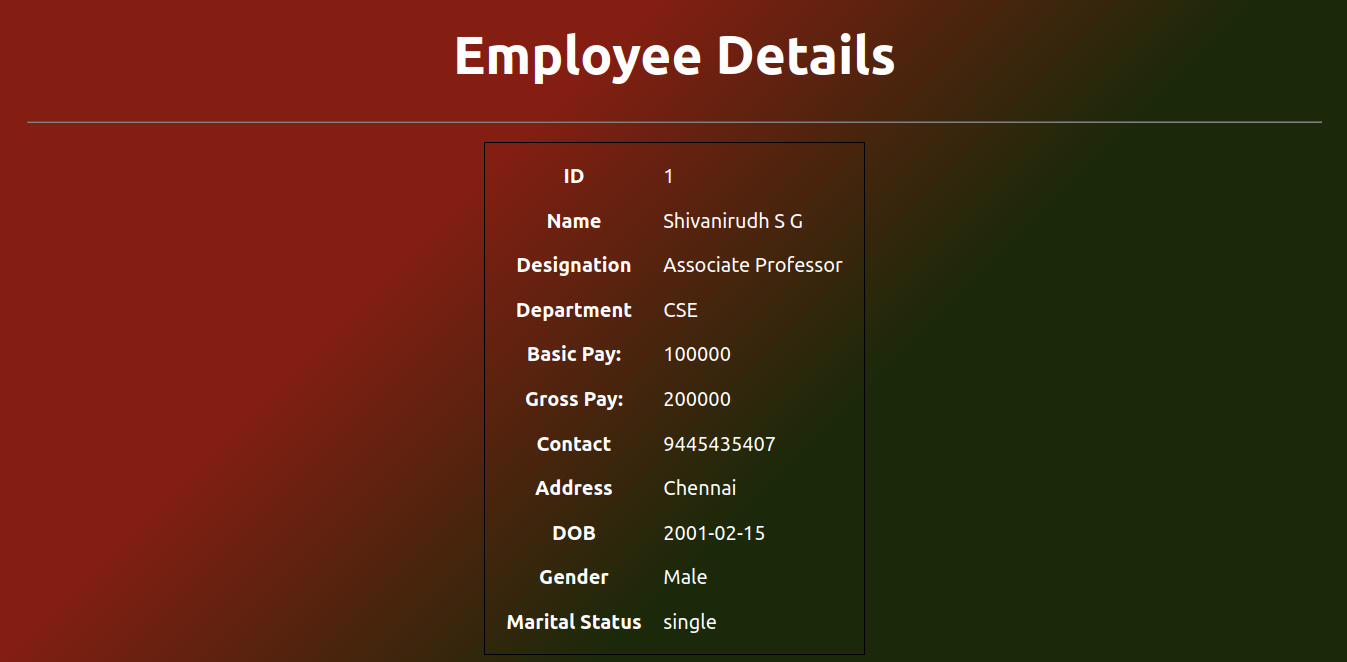
\includegraphics[width = \textwidth]{Pics/reg2.png}
\end{figure}

\hrule

\subsection*{\flushleft{Learning Outcomes:}}
\renewcommand{\labelitemi}{$\textendash$}
\begin{itemize}
    \item Learnt to build a servlet with Apache Tomcat and Java.
    \item Learnt to use servlets to control behaviour of forms.
    \item Learnt to use \textbf{action} tag for loading servlet.
    \item Learnt the different types of getting info from HTML forms in Java.
    \item Learnt to use styling, and behaviour of HTML items in Java.
\end{itemize}
\hrule
\end{document}